% Supplementary material for the ACCV 2026 TrustFMI submission "Protect the Decoder".
% Same class and conventions as main.tex; double-blind, no names or links.
\documentclass[runningheads]{llncs}
\usepackage{graphicx}
\usepackage{booktabs}
\usepackage{amsmath,amssymb}
\usepackage{multirow}
\usepackage[hidelinks]{hyperref}
\renewcommand{\thetable}{S\arabic{table}}
\renewcommand{\thefigure}{S\arabic{figure}}
\renewcommand{\thesection}{S\arabic{section}}

\begin{document}

\title{Supplementary Material:\\Protect the Decoder: Representation-Preserving Adaptation and Failure Detection for Far-OOD MedSAM}
\titlerunning{Protect the Decoder: Supplement}
\author{Anonymous Submission}
\authorrunning{Anonymous}
\institute{}

\maketitle

This supplement holds the tables and figures the main text refers to: the prompt-robustness numbers behind the six-curve figure with their paired tests (Sect.~\ref{sup:robust}), the held-out DMID results (Sect.~\ref{sup:dmid}), the 50\,px failure-detection table (Sect.~\ref{sup:pm50}), the failure-threshold sensitivity check (Sect.~\ref{sup:thresh}), the risk-coverage analysis behind the review-budget numbers (Sect.~\ref{sup:rc}), and the calibration of the decoder's IoU estimate (Sect.~\ref{sup:cal}). All numbers are produced by the released scripts from the per-image result files.

\section{Prompt robustness per expansion level}
\label{sup:robust}

Table~\ref{tab:sup_robust} lists the Dice values plotted in the main text's six-curve figure: LoRA with and without the decoder CKA loss under three training regimes (tight boxes, 20\,px jitter, random jitter up to 100\,px), evaluated with boxes expanded outward by up to 0, 20, 50, 100 and 200\,px. Entries with a standard deviation are means over seeds 0 to 2; the others are seed 0. Table~\ref{tab:sup_wilcoxon} gives the paired Wilcoxon signed-rank test between the two 20\,px-trained models at each level, pairs matched on seed and image, with Holm correction over the four datasets at each level.

\begin{table}[htbp]
  \centering
  \caption{Dice against box expansion for the six models of the main text's robustness figure. Mean $\pm$ std over three seeds where available.}
  \label{tab:sup_robust}
  \scriptsize
  \begin{tabular}{llccccc}
\toprule
Model & Dataset & 0\,px & 20\,px & 50\,px & 100\,px & 200\,px \\
\midrule
no-CKA pm0 & ISIC (ID) & 0.956 $\pm$ 0.001 & 0.942 $\pm$ 0.002 & 0.904 $\pm$ 0.004 & 0.852 $\pm$ 0.007 & 0.787 $\pm$ 0.012 \\
no-CKA pm0 & PH2 (near-OOD) & 0.957 $\pm$ 0.001 & 0.938 $\pm$ 0.001 & 0.904 $\pm$ 0.004 & 0.860 $\pm$ 0.009 & 0.820 $\pm$ 0.015 \\
no-CKA pm0 & BUSI (far-OOD) & 0.780 $\pm$ 0.002 & 0.754 $\pm$ 0.002 & 0.697 $\pm$ 0.002 & 0.619 $\pm$ 0.004 & 0.490 $\pm$ 0.006 \\
no-CKA pm0 & CBIS-DDSM (far-OOD) & 0.509 $\pm$ 0.010 & 0.478 $\pm$ 0.015 & 0.388 $\pm$ 0.013 & 0.270 $\pm$ 0.014 & 0.147 $\pm$ 0.004 \\
no-CKA pm20 & ISIC (ID) & 0.949 $\pm$ 0.002 & 0.939 $\pm$ 0.001 & 0.911 $\pm$ 0.004 & 0.863 $\pm$ 0.009 & 0.797 $\pm$ 0.015 \\
no-CKA pm20 & PH2 (near-OOD) & 0.951 $\pm$ 0.001 & 0.938 $\pm$ 0.003 & 0.913 $\pm$ 0.006 & 0.872 $\pm$ 0.009 & 0.834 $\pm$ 0.008 \\
no-CKA pm20 & BUSI (far-OOD) & 0.774 $\pm$ 0.032 & 0.759 $\pm$ 0.034 & 0.716 $\pm$ 0.035 & 0.635 $\pm$ 0.030 & 0.501 $\pm$ 0.017 \\
no-CKA pm20 & CBIS-DDSM (far-OOD) & 0.437 $\pm$ 0.095 & 0.419 $\pm$ 0.083 & 0.358 $\pm$ 0.062 & 0.247 $\pm$ 0.029 & 0.133 $\pm$ 0.008 \\
no-CKA rand100 & ISIC (ID) & 0.941 $\pm$ 0.002 & 0.937 $\pm$ 0.004 & 0.926 $\pm$ 0.006 & 0.902 $\pm$ 0.006 & 0.848 $\pm$ 0.002 \\
no-CKA rand100 & PH2 (near-OOD) & 0.950 $\pm$ 0.004 & 0.944 $\pm$ 0.005 & 0.933 $\pm$ 0.006 & 0.910 $\pm$ 0.005 & 0.877 $\pm$ 0.004 \\
no-CKA rand100 & BUSI (far-OOD) & 0.747 $\pm$ 0.032 & 0.740 $\pm$ 0.036 & 0.716 $\pm$ 0.040 & 0.654 $\pm$ 0.045 & 0.496 $\pm$ 0.032 \\
no-CKA rand100 & CBIS-DDSM (far-OOD) & 0.214 $\pm$ 0.034 & 0.224 $\pm$ 0.020 & 0.215 $\pm$ 0.020 & 0.168 $\pm$ 0.030 & 0.095 $\pm$ 0.020 \\
CKA pm0 & ISIC (ID) & 0.953 & 0.936 & 0.891 & 0.822 & 0.720 \\
CKA pm0 & PH2 (near-OOD) & 0.952 & 0.932 & 0.893 & 0.830 & 0.748 \\
CKA pm0 & BUSI (far-OOD) & 0.871 & 0.862 & 0.805 & 0.702 & 0.545 \\
CKA pm0 & CBIS-DDSM (far-OOD) & 0.779 & 0.714 & 0.517 & 0.292 & 0.146 \\
CKA pm20 & ISIC (ID) & 0.952 $\pm$ 0.002 & 0.942 $\pm$ 0.003 & 0.911 $\pm$ 0.002 & 0.850 $\pm$ 0.004 & 0.764 $\pm$ 0.008 \\
CKA pm20 & PH2 (near-OOD) & 0.954 $\pm$ 0.002 & 0.942 $\pm$ 0.002 & 0.912 $\pm$ 0.001 & 0.861 $\pm$ 0.001 & 0.800 $\pm$ 0.002 \\
CKA pm20 & BUSI (far-OOD) & 0.826 $\pm$ 0.008 & 0.811 $\pm$ 0.013 & 0.762 $\pm$ 0.019 & 0.672 $\pm$ 0.023 & 0.518 $\pm$ 0.023 \\
CKA pm20 & CBIS-DDSM (far-OOD) & 0.541 $\pm$ 0.095 & 0.507 $\pm$ 0.077 & 0.410 $\pm$ 0.059 & 0.255 $\pm$ 0.031 & 0.134 $\pm$ 0.014 \\
CKA rand100 & ISIC (ID) & 0.941 & 0.937 & 0.927 & 0.904 & 0.851 \\
CKA rand100 & PH2 (near-OOD) & 0.947 & 0.943 & 0.934 & 0.914 & 0.880 \\
CKA rand100 & BUSI (far-OOD) & 0.688 & 0.675 & 0.644 & 0.585 & 0.466 \\
CKA rand100 & CBIS-DDSM (far-OOD) & 0.183 & 0.185 & 0.164 & 0.128 & 0.081 \\
\bottomrule
\end{tabular}

\end{table}

\begin{table}[htbp]
  \centering
  \caption{Paired per-image Dice difference, CKA minus no-CKA (both 20\,px training), at each evaluation level. Improved: fraction of pairs with a positive difference.}
  \label{tab:sup_wilcoxon}
  \scriptsize
  \begin{tabular}{lrrrrrr}
\toprule
Dataset & Level (px) & Pairs & Mean $\Delta$ & Median $\Delta$ & Improved & $p$ (Holm) \\
\midrule
ISIC (ID) & 20 & 3000 & +0.003 & +0.002 & 58\% & $<$0.001 \\
ISIC (ID) & 50 & 3000 & -0.001 & -0.001 & 49\% & 0.084 \\
ISIC (ID) & 100 & 3000 & -0.013 & -0.010 & 34\% & $<$0.001 \\
ISIC (ID) & 200 & 3000 & -0.033 & -0.027 & 24\% & $<$0.001 \\
PH2 (near-OOD) & 20 & 600 & +0.004 & +0.003 & 59\% & $<$0.001 \\
PH2 (near-OOD) & 50 & 600 & -0.001 & -0.000 & 49\% & 0.483 \\
PH2 (near-OOD) & 100 & 600 & -0.011 & -0.009 & 34\% & $<$0.001 \\
PH2 (near-OOD) & 200 & 600 & -0.033 & -0.026 & 17\% & $<$0.001 \\
BUSI (far-OOD) & 20 & 1941 & +0.053 & +0.012 & 57\% & $<$0.001 \\
BUSI (far-OOD) & 50 & 1941 & +0.046 & +0.014 & 59\% & $<$0.001 \\
BUSI (far-OOD) & 100 & 1941 & +0.038 & +0.020 & 61\% & $<$0.001 \\
BUSI (far-OOD) & 200 & 1941 & +0.017 & +0.010 & 57\% & $<$0.001 \\
CBIS-DDSM (far-OOD) & 20 & 1086 & +0.088 & +0.088 & 64\% & $<$0.001 \\
CBIS-DDSM (far-OOD) & 50 & 1086 & +0.052 & +0.054 & 60\% & $<$0.001 \\
CBIS-DDSM (far-OOD) & 100 & 1086 & +0.008 & +0.015 & 55\% & 0.014 \\
CBIS-DDSM (far-OOD) & 200 & 1086 & +0.001 & +0.004 & 54\% & 0.369 \\
\bottomrule
\end{tabular}

\end{table}

\section{Held-out mammography set (DMID)}
\label{sup:dmid}

DMID was used once, after every model and every hyperparameter was fixed. Table~\ref{tab:sup_dmid} reports tight-box Dice and HD95 on its 269 annotated mammograms for the seven strategies and the CKA-regularised LoRA variants; the ranking matches CBIS-DDSM in every comparison made in the main text. The row marked $n=2$ is the mean of seeds 1 and 2 of that configuration.

\begin{table}[htbp]
  \centering
  \caption{DMID, tight boxes, 269 images. HD95 in pixels on the 1024 grid.}
  \label{tab:sup_dmid}
  \begin{tabular}{lcc}
\toprule
Method & Dice & HD95 (px) \\
\midrule
Zero-shot & 0.637 & 30 \\
Decoder-only FT & 0.727 & 32 \\
VPT-shallow & 0.572 & 217 \\
VPT-deep & 0.526 & 253 \\
LoRA & 0.402 & 319 \\
Encoder-only LoRA & 0.733 & 25 \\
Full FT & 0.727 & 25 \\
LoRA + CKA (decoder hooks, tight training) & 0.697 & 65 \\
LoRA + CKA (decoder hooks, 20 px) ($n=2$) & 0.556 & 120 \\
LoRA + CKA (encoder hooks, 20 px) & 0.366 & 330 \\
LoRA + CKA (both, 20 px) & 0.651 & 94 \\
\bottomrule
\end{tabular}

\end{table}

\section{Failure detection under 50\,px box jitter}
\label{sup:pm50}

Table~\ref{tab:sup_pm50} repeats the main text's detector table with boxes expanded by up to 50\,px, the setting in which full fine-tuning and encoder-only LoRA produce enough failures to be scored on the ladder. The IoU estimate detects these prompt-induced failures for every method while drift does not, the pattern discussed in the main text.

\begin{table}[htbp]
  \centering
  \caption{AUROC / AUPRC for detecting per-image failures (Dice below 0.5) at 50\,px box jitter. Cells with fewer than 20 failures omitted; drift is zero by construction for zero-shot.}
  \label{tab:sup_pm50}
  \begin{tabular}{lcccc}
\toprule
Method & \multicolumn{2}{c}{BUSI (far-OOD)} & \multicolumn{2}{c}{CBIS-DDSM (far-OOD)} \\
 & drift & IoU head & drift & IoU head \\
\midrule
Zero-shot & -- & 0.87 & -- & 0.71 \\
Decoder-only FT & 0.79 & 0.48 & 0.55 & 0.58 \\
VPT-shallow & 0.92 & 0.49 & 0.71 & 0.36 \\
VPT-deep & 0.93 & 0.63 & 0.61 & 0.59 \\
LoRA & 0.91 & 0.69 & 0.76 & 0.44 \\
Encoder-only LoRA & 0.35 & 0.89 & 0.36 & 0.75 \\
Full FT & 0.23 & 0.87 & 0.32 & 0.79 \\
\bottomrule
\end{tabular}

\end{table}

\section{Sensitivity to the failure threshold}
\label{sup:thresh}

The main text defines a failure as Dice below 0.5. Tables~\ref{tab:sup_thresh0} and~\ref{tab:sup_thresh50} recompute the drift AUROC for LoRA and the two VPT variants with the threshold moved from 0.3 to 0.7, at tight boxes and at 50\,px jitter. The ordering of methods and datasets is unchanged at every threshold, and LoRA's values stay within 0.90 to 0.97 on BUSI and 0.73 to 0.82 on CBIS-DDSM at tight boxes.

\begin{table}[htbp]
  \centering
  \caption{Drift AUROC as a function of the Dice threshold that defines a failure, tight boxes.}
  \label{tab:sup_thresh0}
  \begin{tabular}{llccccc}
\toprule
Method & Dataset & 0.3 & 0.4 & 0.5 & 0.6 & 0.7 \\
\midrule
VPT-shallow & BUSI (far-OOD) & 0.93 & 0.94 & 0.93 & 0.93 & 0.88 \\
VPT-shallow & CBIS-DDSM (far-OOD) & 0.59 & 0.65 & 0.70 & 0.70 & 0.71 \\
VPT-deep & BUSI (far-OOD) & 0.92 & 0.90 & 0.92 & 0.90 & 0.84 \\
VPT-deep & CBIS-DDSM (far-OOD) & 0.62 & 0.65 & 0.66 & 0.68 & 0.70 \\
LoRA & BUSI (far-OOD) & 0.97 & 0.94 & 0.95 & 0.93 & 0.90 \\
LoRA & CBIS-DDSM (far-OOD) & 0.81 & 0.82 & 0.82 & 0.77 & 0.73 \\
\bottomrule
\end{tabular}

\end{table}

\begin{table}[htbp]
  \centering
  \caption{As Table~\ref{tab:sup_thresh0}, at 50\,px box jitter.}
  \label{tab:sup_thresh50}
  \begin{tabular}{llccccc}
\toprule
Method & Dataset & 0.3 & 0.4 & 0.5 & 0.6 & 0.7 \\
\midrule
VPT-shallow & BUSI (far-OOD) & 0.92 & 0.91 & 0.92 & 0.90 & 0.88 \\
VPT-shallow & CBIS-DDSM (far-OOD) & 0.66 & 0.68 & 0.71 & 0.71 & 0.65 \\
VPT-deep & BUSI (far-OOD) & 0.90 & 0.91 & 0.93 & 0.90 & 0.87 \\
VPT-deep & CBIS-DDSM (far-OOD) & 0.61 & 0.61 & 0.61 & 0.63 & 0.57 \\
LoRA & BUSI (far-OOD) & 0.91 & 0.91 & 0.91 & 0.91 & 0.90 \\
LoRA & CBIS-DDSM (far-OOD) & 0.73 & 0.75 & 0.76 & 0.76 & 0.71 \\
\bottomrule
\end{tabular}

\end{table}

\section{Risk-coverage analysis}
\label{sup:rc}

Ranking images by drift and flagging the top fraction for review gives, for each budget, the recall of failures among the flagged images and the failure rate that remains among the unflagged ones (the selective risk). Table~\ref{tab:sup_rc} lists both at four review budgets, together with the base failure rate and the area under the risk-coverage curve (AURC), for which a random ranking scores the base rate. Figure~\ref{fig:sup_rc} shows the full curves for drift (solid) and the IoU estimate (dashed).

\begin{table}[htbp]
  \centering
  \caption{Tight boxes, failure = Dice below 0.5, ranking by drift. Cells: recall of failures / residual failure rate among unflagged images when the top 10, 20, 30 or 50 percent of images are flagged.}
  \label{tab:sup_rc}
  \scriptsize
  \begin{tabular}{llcccccc}
\toprule
Method & Dataset & Base rate & AURC & top 10\% & top 20\% & top 30\% & top 50\% \\
\midrule
VPT-shallow & BUSI (far-OOD) & 0.043 & 0.004 & 0.79 / 0.010 & 0.86 / 0.008 & 0.89 / 0.007 & 1.00 / 0.000 \\
VPT-shallow & CBIS-DDSM (far-OOD) & 0.215 & 0.176 & 0.29 / 0.169 & 0.47 / 0.142 & 0.59 / 0.126 & 0.73 / 0.116 \\
VPT-deep & BUSI (far-OOD) & 0.068 & 0.009 & 0.55 / 0.034 & 0.86 / 0.012 & 0.91 / 0.009 & 0.98 / 0.003 \\
VPT-deep & CBIS-DDSM (far-OOD) & 0.312 & 0.265 & 0.24 / 0.265 & 0.36 / 0.249 & 0.50 / 0.221 & 0.66 / 0.210 \\
LoRA & BUSI (far-OOD) & 0.094 & 0.010 & 0.70 / 0.031 & 0.87 / 0.015 & 0.93 / 0.009 & 1.00 / 0.000 \\
LoRA & CBIS-DDSM (far-OOD) & 0.420 & 0.258 & 0.24 / 0.354 & 0.45 / 0.287 & 0.61 / 0.233 & 0.79 / 0.177 \\
\bottomrule
\end{tabular}

\end{table}

\begin{figure}[htbp]
  \centering
  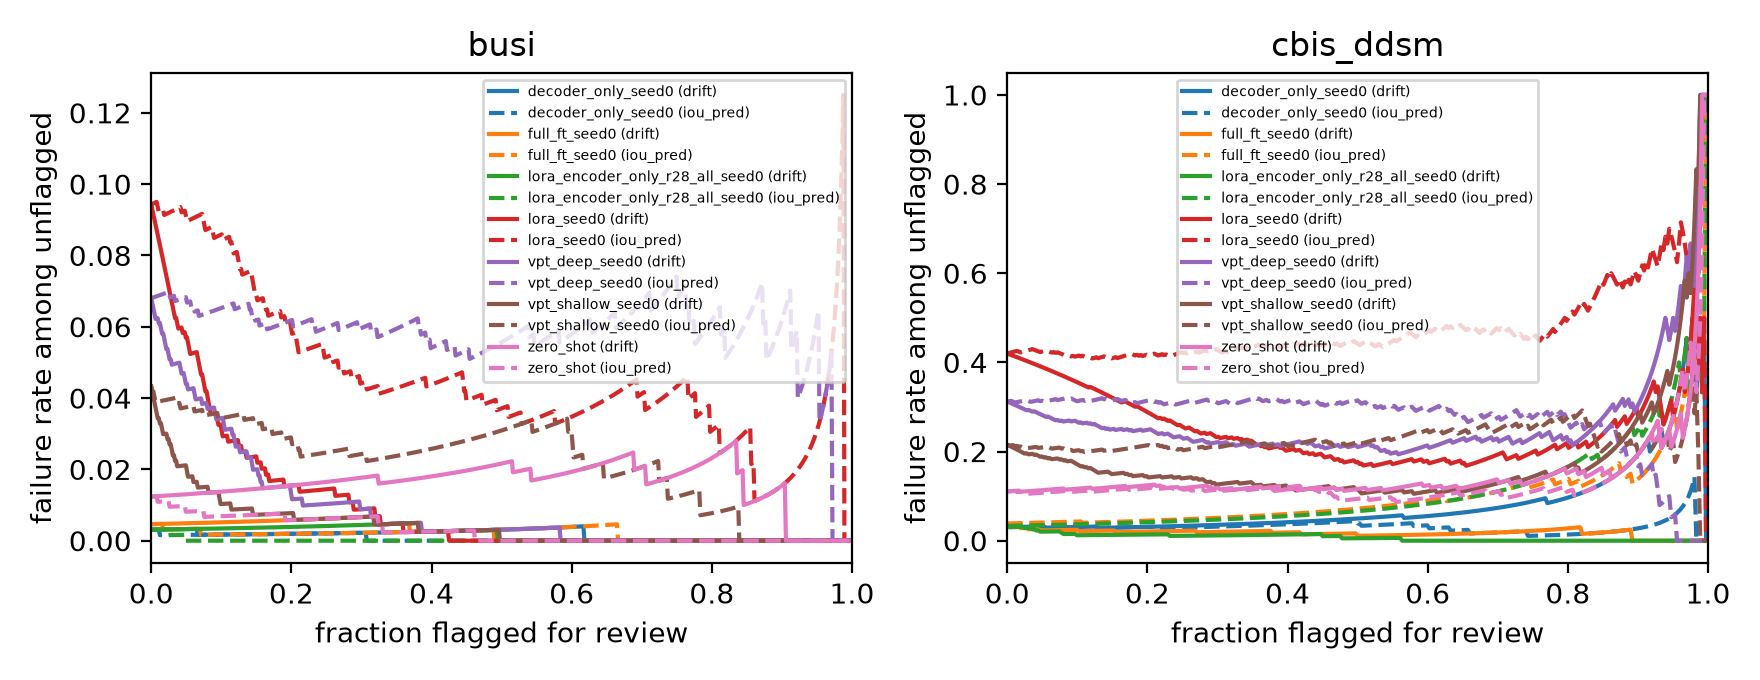
\includegraphics[width=0.95\linewidth]{figures/risk_coverage_pm0.png}
  \caption{Residual failure rate among unflagged images against the fraction flagged, tight boxes, for drift (solid) and the negated IoU estimate (dashed). A curve that falls quickly leaves few failures unreviewed.}
  \label{fig:sup_rc}
\end{figure}

\section{Calibration of the IoU estimate}
\label{sup:cal}

Tables~\ref{tab:sup_cal0} and~\ref{tab:sup_cal50} give the ten-bin expected calibration error of the decoder's IoU estimate $\hat{u}$ against the true IoU on the two far-OOD sets, with the mean of each. After adaptation the estimate sits near 0.5 regardless of the true value; Fig.~\ref{fig:sup_scatter} shows the collapse for LoRA at tight boxes.

\begin{table}[htbp]
  \centering
  \caption{Calibration of the IoU estimate at tight boxes: expected calibration error, mean predicted IoU $\hat{u}$, mean true IoU.}
  \label{tab:sup_cal0}
  \begin{tabular}{lcccccc}
\toprule
Method & \multicolumn{3}{c}{BUSI (far-OOD)} & \multicolumn{3}{c}{CBIS-DDSM (far-OOD)} \\
 & ECE & $\hat{u}$ & IoU & ECE & $\hat{u}$ & IoU \\
\midrule
Zero-shot & 0.16 & 0.55 & 0.71 & 0.09 & 0.48 & 0.55 \\
Decoder-only FT & 0.34 & 0.47 & 0.81 & 0.24 & 0.48 & 0.72 \\
VPT-shallow & 0.17 & 0.53 & 0.70 & 0.03 & 0.53 & 0.50 \\
VPT-deep & 0.17 & 0.52 & 0.69 & 0.07 & 0.49 & 0.44 \\
LoRA & 0.16 & 0.51 & 0.67 & 0.13 & 0.50 & 0.38 \\
Encoder-only LoRA & 0.28 & 0.56 & 0.84 & 0.23 & 0.49 & 0.71 \\
Full FT & 0.26 & 0.56 & 0.82 & 0.22 & 0.50 & 0.72 \\
\bottomrule
\end{tabular}

\end{table}

\begin{table}[htbp]
  \centering
  \caption{As Table~\ref{tab:sup_cal0}, at 50\,px box jitter.}
  \label{tab:sup_cal50}
  \begin{tabular}{lcccccc}
\toprule
Method & \multicolumn{3}{c}{BUSI (far-OOD)} & \multicolumn{3}{c}{CBIS-DDSM (far-OOD)} \\
 & ECE & $\hat{u}$ & IoU & ECE & $\hat{u}$ & IoU \\
\midrule
Zero-shot & 0.07 & 0.53 & 0.57 & 0.20 & 0.47 & 0.26 \\
Decoder-only FT & 0.18 & 0.46 & 0.64 & 0.20 & 0.47 & 0.26 \\
VPT-shallow & 0.07 & 0.53 & 0.60 & 0.31 & 0.54 & 0.23 \\
VPT-deep & 0.09 & 0.50 & 0.59 & 0.28 & 0.49 & 0.21 \\
LoRA & 0.06 & 0.51 & 0.57 & 0.31 & 0.50 & 0.20 \\
Encoder-only LoRA & 0.11 & 0.55 & 0.67 & 0.21 & 0.47 & 0.27 \\
Full FT & 0.10 & 0.55 & 0.65 & 0.21 & 0.48 & 0.27 \\
\bottomrule
\end{tabular}

\end{table}

\begin{figure}[htbp]
  \centering
  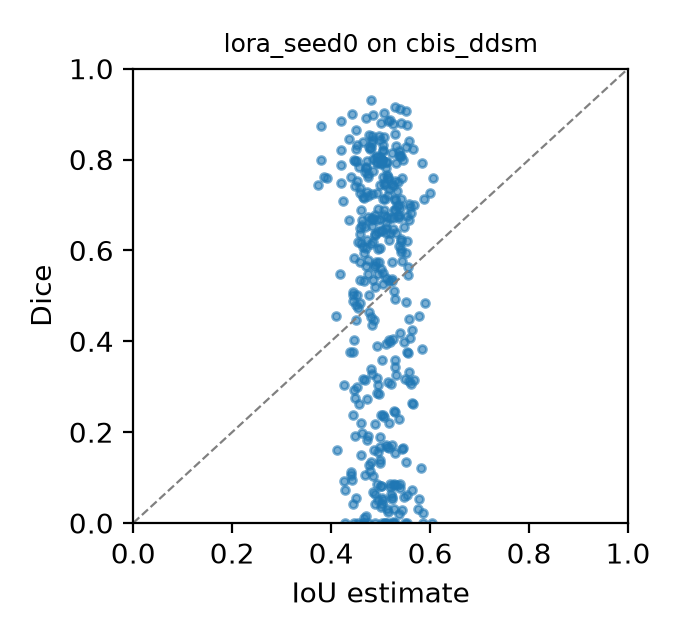
\includegraphics[width=0.7\linewidth]{figures/failure_detection_pm0_scatter.png}
  \caption{Predicted IoU $\hat{u}$ against Dice per image for LoRA on the far-OOD sets at tight boxes. The estimate stays in a band around 0.5 while Dice spans the full range.}
  \label{fig:sup_scatter}
\end{figure}

\end{document}
